Была предпринята попытка замерить время исполнения всех 24 вариаций алгоритмов на следующих операциях:

\begin{itemize}
\item Генерация пары ключей (публичный-приватный)
\item Вычисления хэш-значения
\item Электронная подпись сообщения
\item Верификация сообщения
\item Время работы Proof of Work
\item Время майна одного блока
\end{itemize}

Были замерены время исполнений участков кода готовых реализаций блокчейнв,
сгенерированных при помощи разработанного компоновщика.
Замеры проводились при помощи модуля \emph{time} в Python. Дальнейший анализ и
построение графиков происходило в среде \emph{Jupyter Notebook} с
использованием модуля \underline{matplotlib}.

Была составлена таблица с записями вида \emph{[название алгоритма; функция; битрейт;
время исполнения]} размером более 1500 записей.

\begin{figure}[h!]
    \centering
    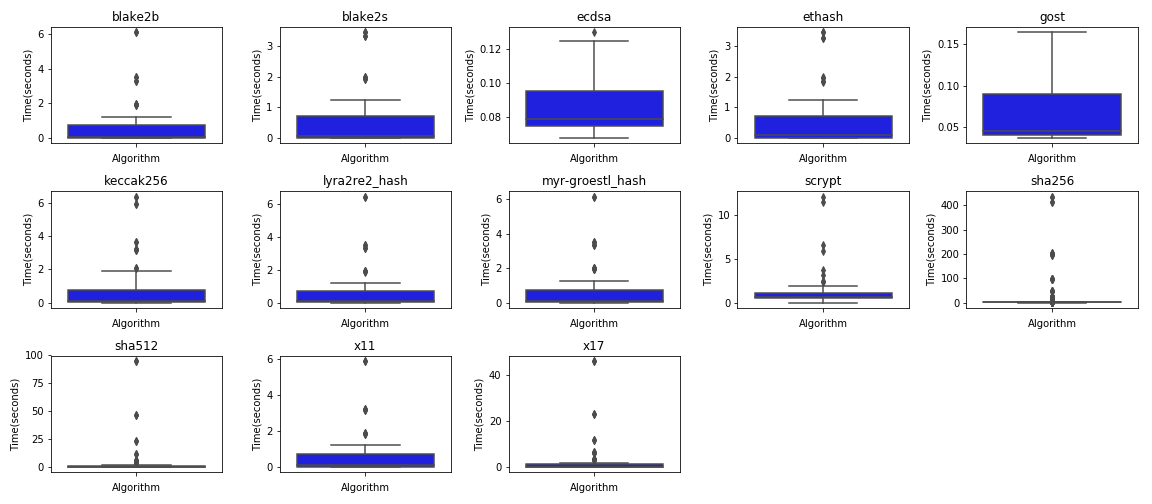
\includegraphics[width=\textwidth]{./images/boxes}
    \caption{Box-plot'ы для распределения алгоритмов по времени}\label{boxes}
\end{figure}

Далее были построены распределения общего вида (Рис. \ref{boxes}), а также
гистограммы распределения времени выполнения для алгоритмов цифровой подписи,
разделяя их на вышеперечисленные процессы (Рис. \ref{dss}):

\begin{figure}[h!]
    \centering
    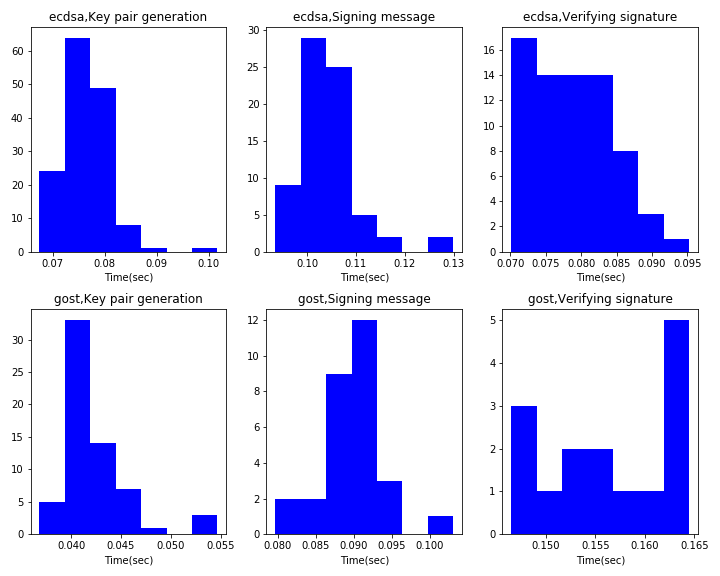
\includegraphics[width=0.68\textwidth]{./images/hists_dss}
    \caption{Распределение времени выполнения среди алгоритмов цифровой подписи}\label{dss}
\end{figure}

И аналогичные данные были построены для алгоритмов хэширования (Рис. \ref{hash}):

\begin{figure}
    \centering
    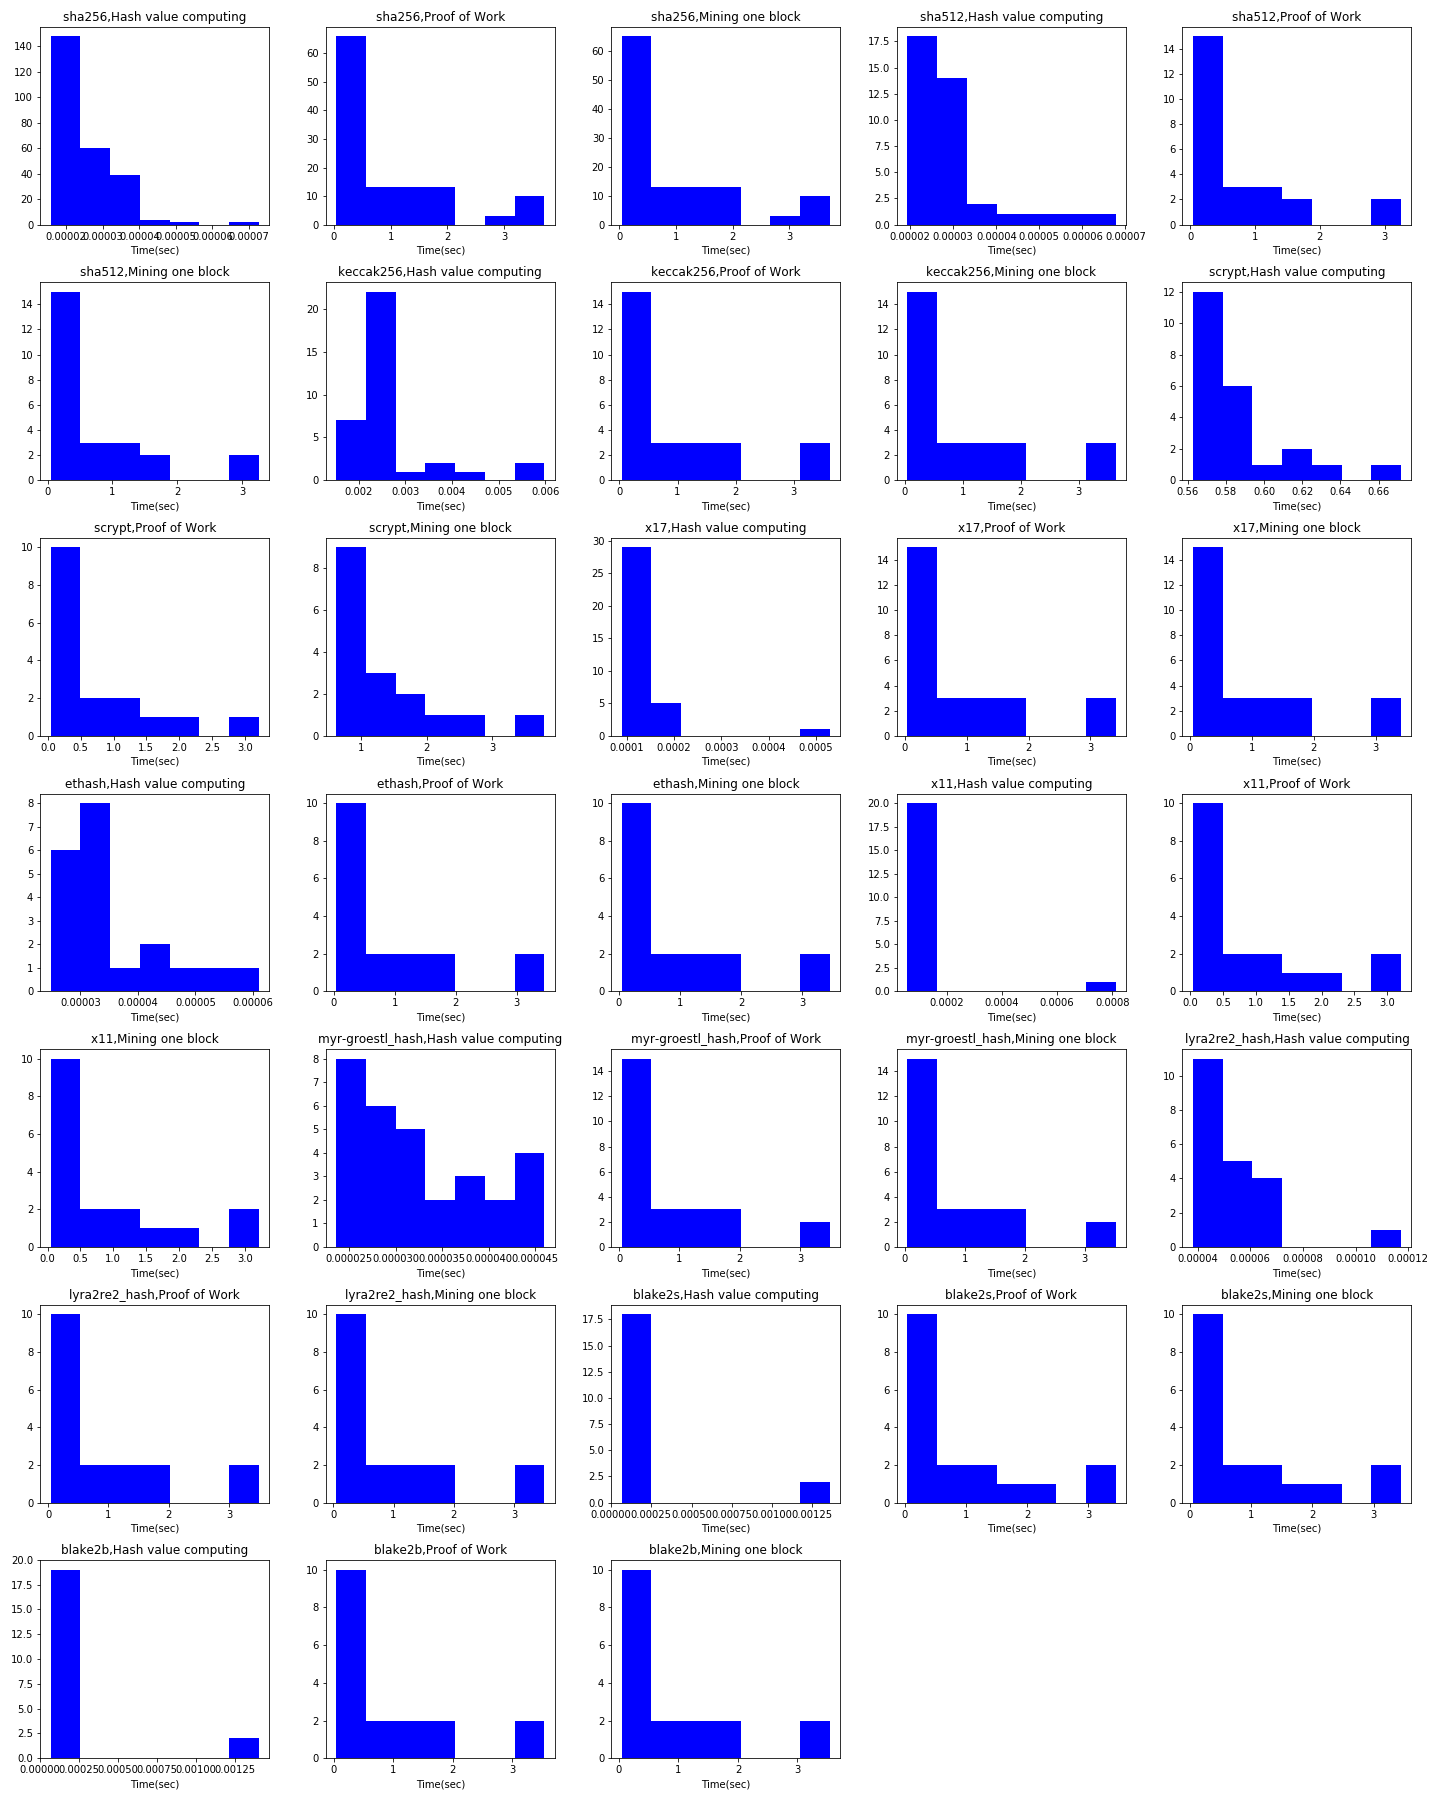
\includegraphics[width=\textwidth]{./images/hists_hashing}
    \caption{Распределение времени выполнения среди алгоритмов хэширования}\label{hash}
\end{figure}

С целью сравнить время исполнения алгоритмов по одинаковым процессам,
расположим их на одном графике гистограммы.  На Рис. \ref{boxes} с бокс-плотами
были видны выбросы, поэтому для усреднения значений на последующих графиках,
были взяты медианы значений, поскольку данные показатель более устойчив к
выбросам, чем обычное среднее.

\begin{figure}[h!]
    \centering
    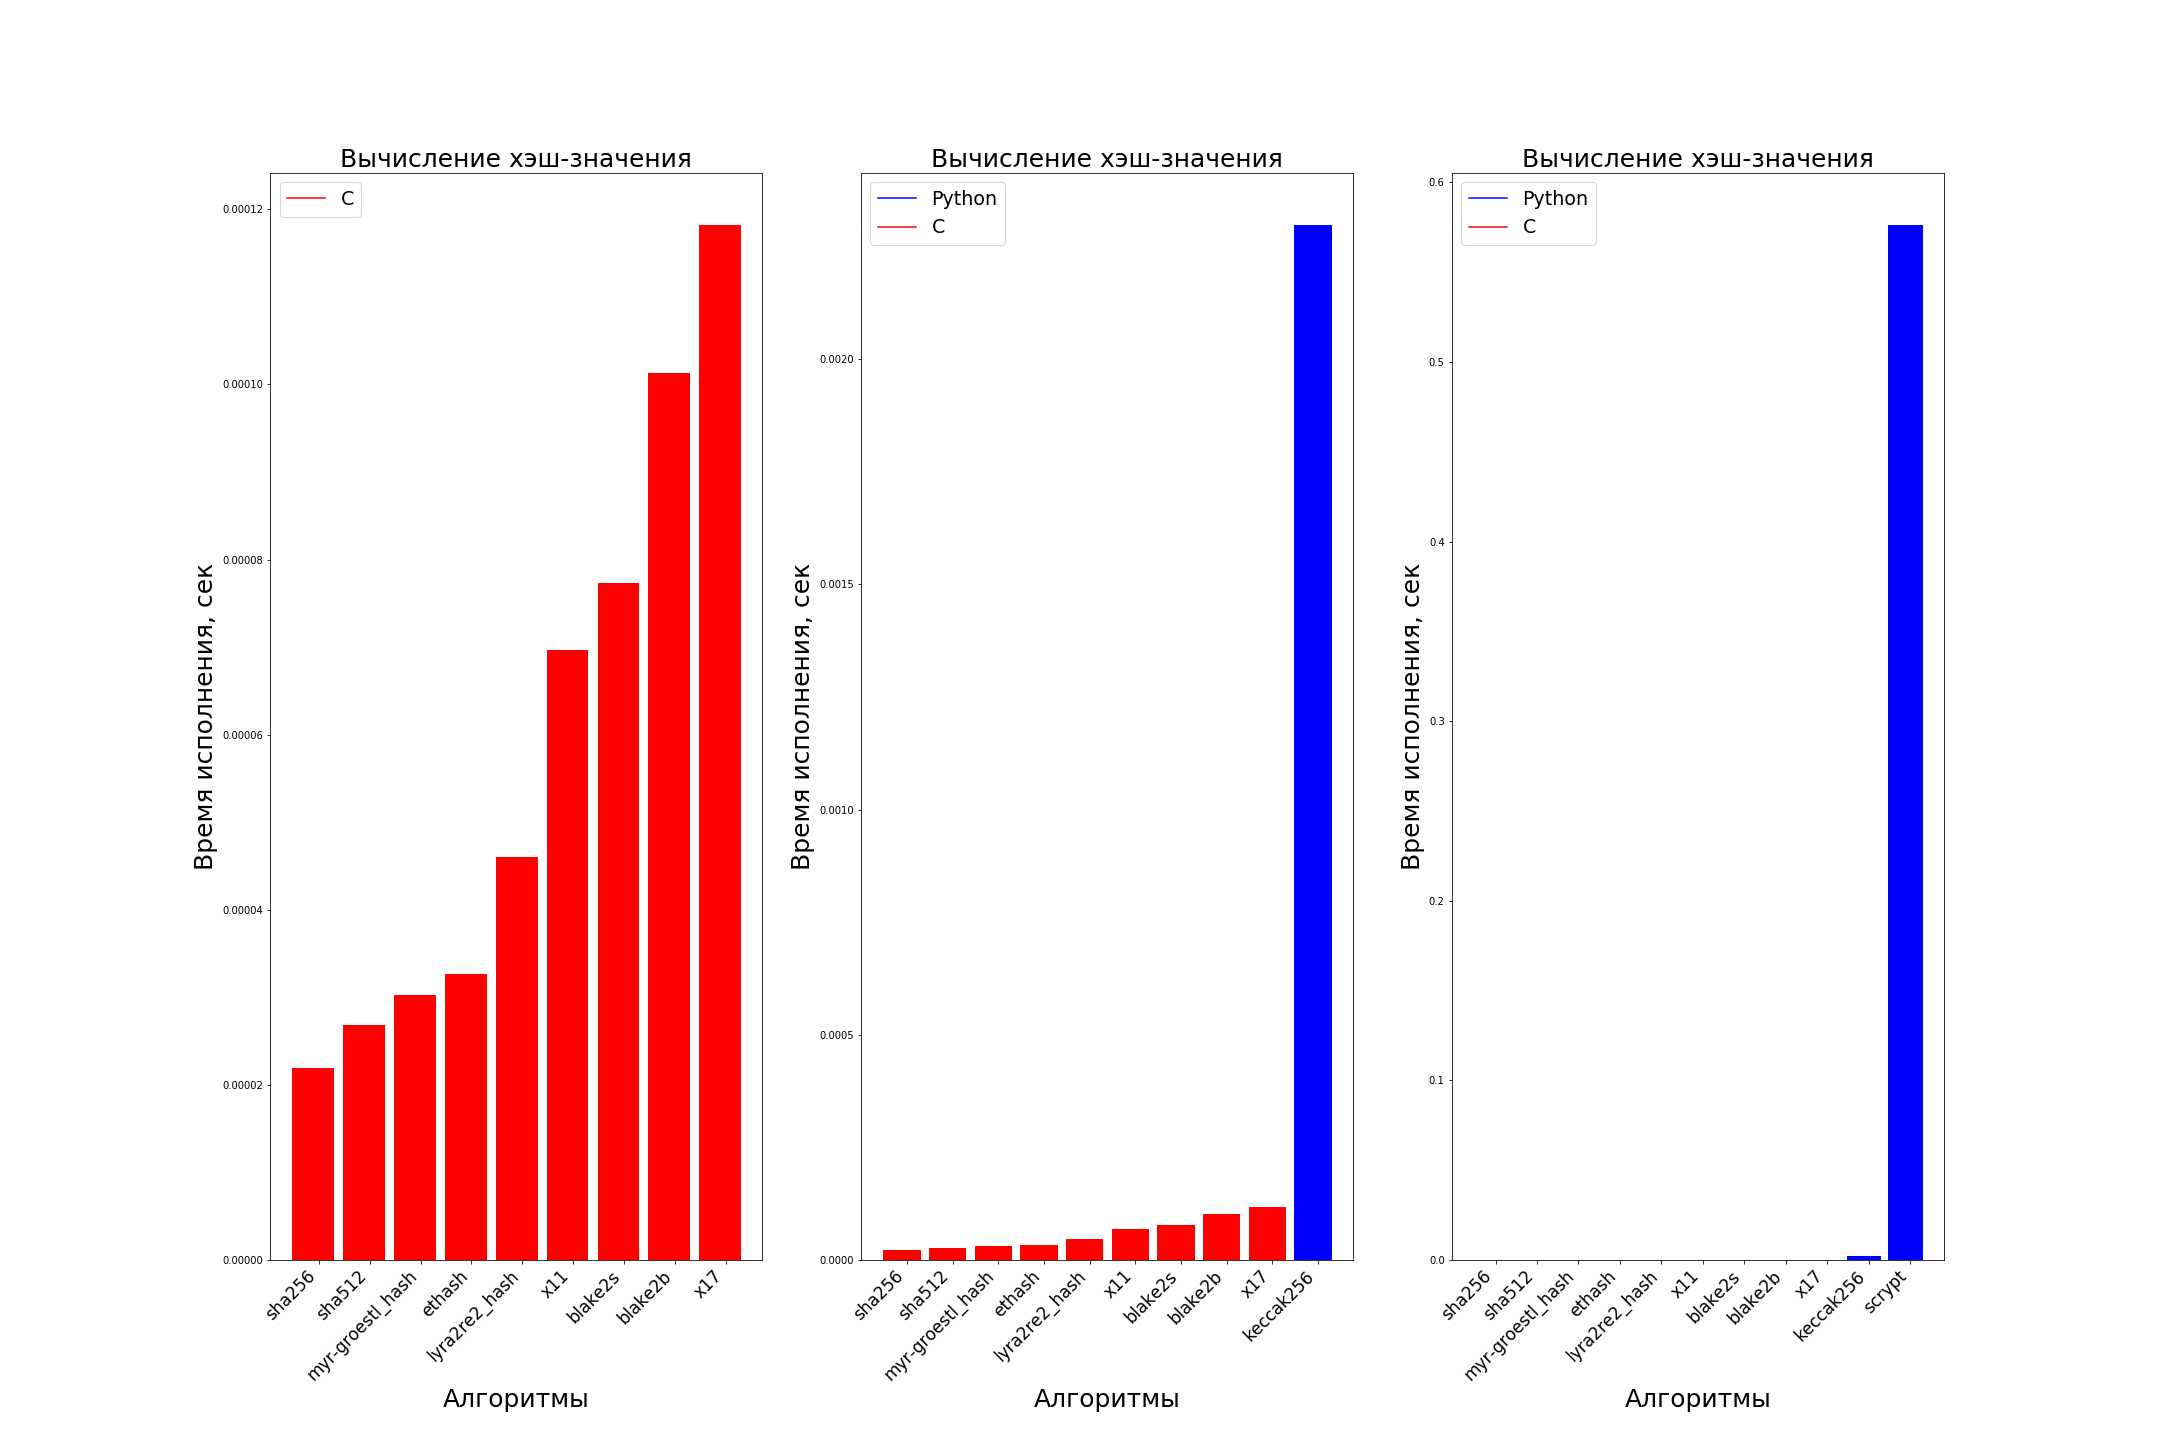
\includegraphics[width=\textwidth]{./images/hash_comparison}
    \caption{Сравнение времени исполнения работ различных алгоритмов хэширования на одинаковых функциях}\label{hash_comp}
\end{figure}

Самым быстрым алгоритмом хэширования \emph{среди упомянутых}, исходя из
проведённого анализа, является, SHA-256. Самым медленным из реализованных на
языке СИ --- X17.  На данных графиках интересно заметить, что оба алгоритма,
реализованные на языке Python, имеют гораздо большее время исполнения, по
сравнению с реализованными на языке СИ. Алгоритм ГОСТ 34.10-2012 проигрывает
международно известной ECSDA лишь во времени исполнения процедуры
верификации (Рис. \ref{dss_comp}).

\begin{figure}[h!]
    \centering
    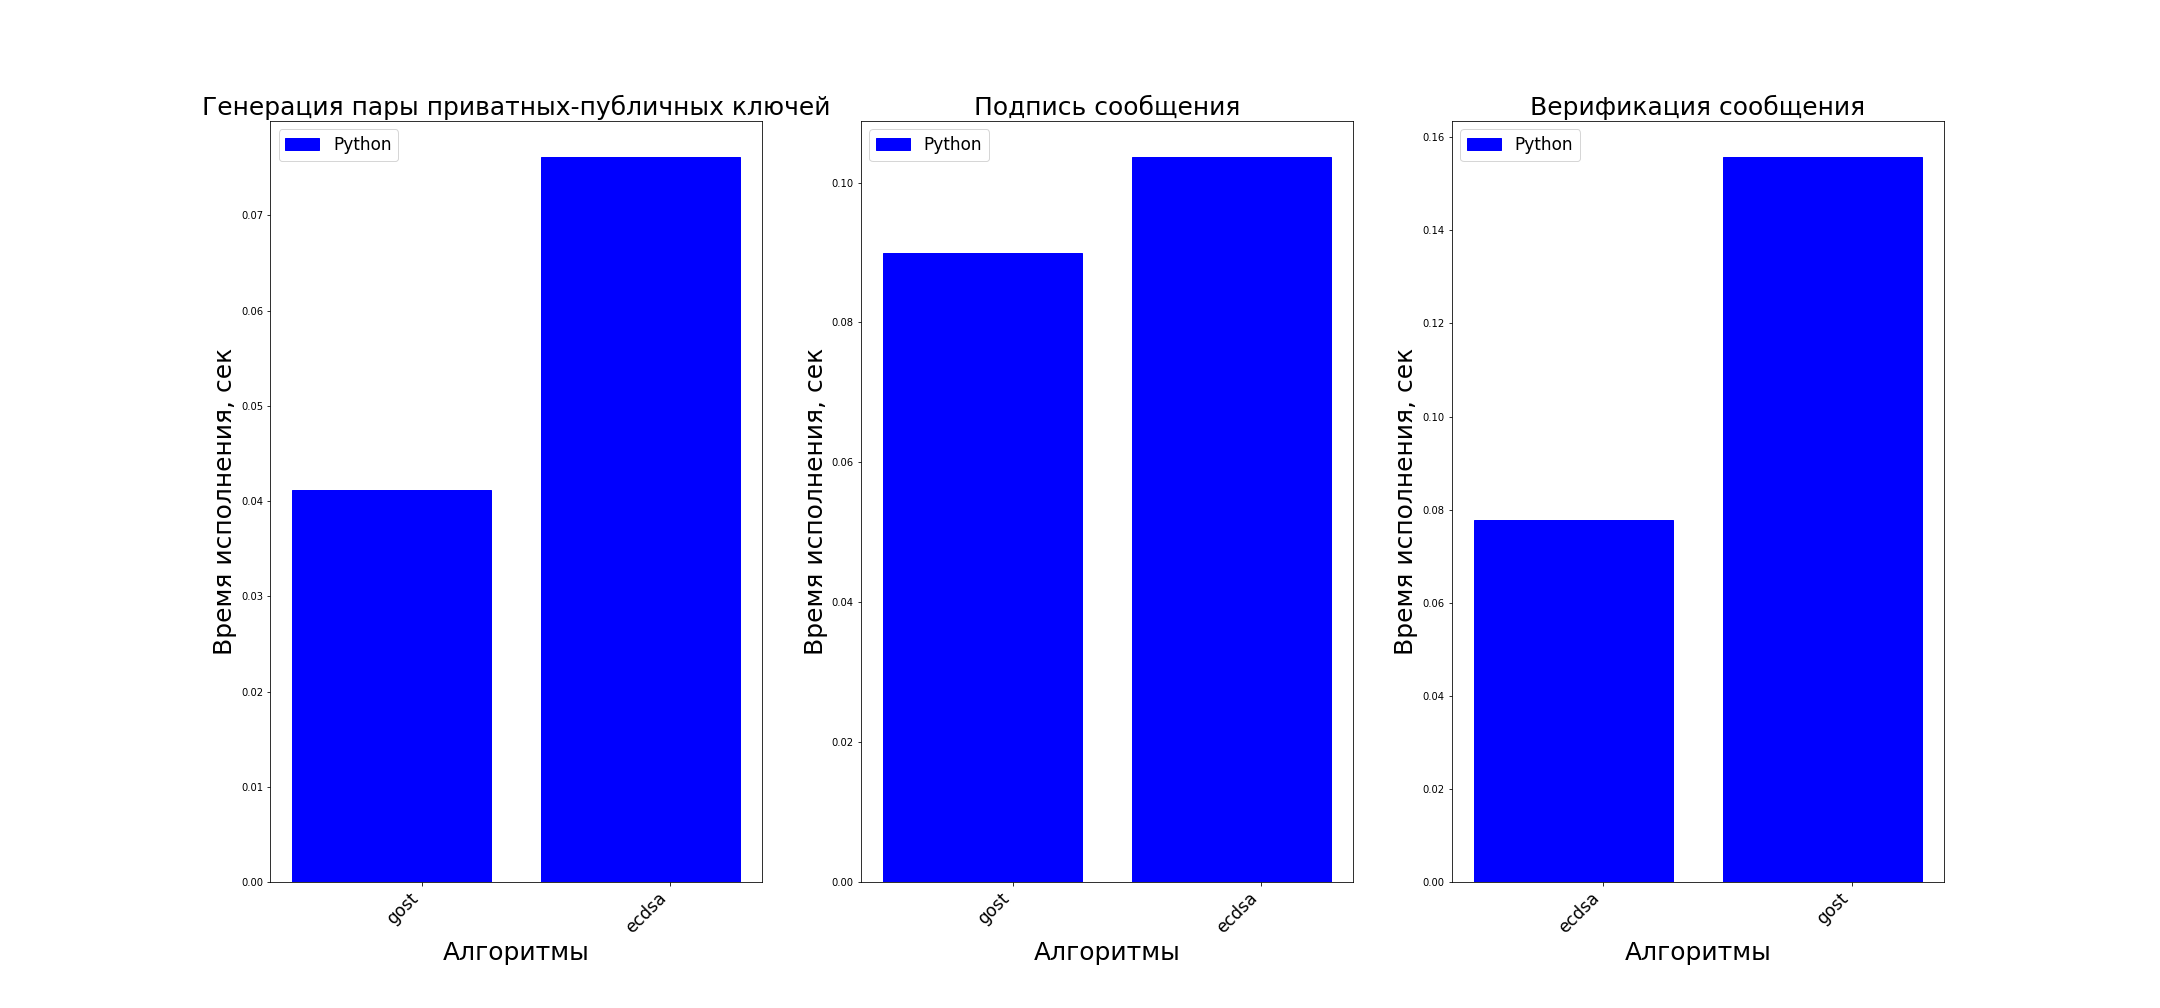
\includegraphics[width=1.\textwidth]{./images/dss_comparison}
    \caption{Сравнение времени исполнения работ различных алгоритмов цифровой подписи на одинаковых функциях}\label{dss_comp}
\end{figure}

